\chapter{Introducci\'on}\label{cap.introduccion}
\hspace{1 cm}Cada vez es mas com\'un el uso de drones para labores que pueden ser muy diversas, como puede ser grabar un plano para una pel\'icula o mantener vigilado un lugar sobrevolando estas zonas. Pero un area muy importante es la navegaci\'on autonoma de estos, conseguir que realicen ciertas tareas sin que haya nadie controlando su ruta ni como se realiza esta. Para ello, hay que contar con los distintos sensores que se le pueden a~nadir a un drone y la forma de utilizar estos en beneficio propio para conseguir dicha navegaci\'on.

\hspace{1cm} En los siguientes parrafos se va a realizar una breve introducci\'on sobre estos aparatos, la historia que tienen, su hardware y software principal y los distintos usos que hay para ellos actualmente.

\section{Historia de los drones}

\hspace{1cm} Los drones son conocidos como UAV(veh\'iculos aereos no tripulados).El primer registro de UAV se trata de un globo aeroest\'atico en un entorno militar, ya que este se pod\'ia utilizar para sobrevolar una zona y lanzar bombas desde cierta altura sin necesidad de que hubiera ninguna persona en este y, por tanto, sin arriesgar una vida. Este UAV es muy distinto a lo que vino despues, principalmente porque el motor de \'este se trata de una bolsa que tiene un gas mas ligero que el aire, lo que le permite coger altura y jugar con las corrientes de viento para desplazarse en una direcci\'on o en otra.

\hspace{1 cm} Mas adelante, ya en la primera guerra mundial, se comenzaron a utilizar para sobrevolar las areas enemigas y hacer fotos de estas para as\'i tener un control de sus movimientos (en este punto nos damos cuenta de que el introducir una c\'amara en un UAV es algo que se hizo desde los primeros momentos, pero en ello ya profundizaremos mas adelante). Estos veh\'iculos eran aviones tripulados por radiofrecuencia, por lo que se dio un gran salto con respecto al anterior, pues era mucho mas facil su control, por lo que pod\'ian manejar su trayectoria con mucha mas facilidad. 

\hspace{1cm} Tambi\'en durante la primera, pero mas desarollado para la segunda guerra mundial, se le di\'o uso a \'estos para utilizarlos como explosivos, ya que pod\'ian seguir su trayectoria en todo momento y asegurarse que llegaban al destino correcto. Adem\'as de poder segir a otros veh\'iculos en movimiento del bando enemigo y as\'i hacer que este no llegara a su destino. 

\hspace{1cm} Est\'a claro que los inicios de estos ten\'ian solo fines militares y que su desarrollo era exclusivamente para ello. En comparaci\'on con estos datos, el avance sobre estos freno en gran medida y ya lo que se hac\'ia era modificaciones para poder dar uso a lo que ya hab\'ia, pues se utilizaban para vigilancia a\'erea en zonas de conflictos, lo que llev\'o a mejorar el sistema de control haciendo as\'i que se pudieran manejar a una mayor distancia. 

\hspace{1 cm}Destacar que fue alrededor de 1980 cuando se vi\'o que la tecnolog\'a y el software de los UAV eran de gran fiabilidad y se pod\'ian asignar a estas tareas de mayor responsabilidad para no jugarse la vida de los pilotos. Decir como dato curioso, que una vez no estaban los pilotos en la cabina del veh\'iculo se pod\'ia jugar con mayor libertad a la hora de realizar movimientos, ya que ciertos giros que los pilotos no podian realizar por ser demasiado bruscos para aguantarlos el cuerpo humano, ahora pod\'ian hacerlos con la brusquedad que permitiera el sistema.  

\hspace{1 cm} Tras esto ya en la decada de los 90 se da un avance muy importante, y es que se desarrolla el sistema GPS para el desplazamiento de estos veh\'iculos. Esto permit\'ia no depender de la radiofrecuencia, ya que con \'esta vamos a tener un l\'imite en distancia y no revisar los datos para ver en todo momento su situaci\'on y dirigir la trayectoria. Con \'este sistema se traza una ruta al inicio y el UAV puede trabajar de forma autonoma. 

\hspace{1cm} Con todo esto, y teniendo en cuenta que fue en torno al a~no 2000 cuando se comenzo a dar un uso a los drones tal y como los vemos ahora, no un enfoque tan militar y si mas para uso civil, hay que destacar el gran avance que ha sufrido la rob\'otica aerea, pues en la parte aeroespacial, cada vehiculo innovador que sale mejora con creces el anterior, por cualidades como materiales,  dise~no o estructura, permitiendo esto una mayor velocidad o resistencia. Y por parte de la rob\'otica ocurre lo mismo, se esta en un continuo desarrollo, y viendo el futuro que tienen los drones muchas empresas y grupos de investigaci\'on han decidido centrarse en ellos, pudiendo asi mejorar a diario el software de estos, lo que permite un control mas fluido, gracias al env\'io y procesamiento de informaci\'on, asi como controlar mejor en todo momento el estado que se encuentra el drone(bateria, posicionamiento en los distintos ejes o velocidad). 
 




\section{Hardware.}
\hspace{1 cm} Hay que destacar las partes que tiene un drone y su forma, pues es gran parte lo que lo hace tan especial,permite que tenga una gran libertad de movimientos, ya que puede moverse sin problema desde cualquier punto hacia los ejes X, Y y Z. Lo que ganamos con esto son cosas como poder permitirse un aterrizaje y un despegue totalmente vertical, sin depender de un espacio en el que cojer velocidad para poder levantar el vuelo, e igual con el aterrizaje, pudiendo el dron estando quieto en el aire bajar totalmente en vertical hasta tocar posarse sobre el suelo. Una vez en el aire pueden moverse adelante, atr\'as, izquierda, derecha, arriba, abajo y combinaciones de movimientos entre ejes, adem\'as de los movimientos Roll, Yaw y Pitch y sin necesidad de hacer movimientos bruscos. Sin embargo, en los anteriores UAV solo tenemos el movimiento hacia adelante, teniendo que jugar con Roll, Yaw y Pitch para poder movernos en los distintos ejes.

\begin{figure}[ht]
	\centering
		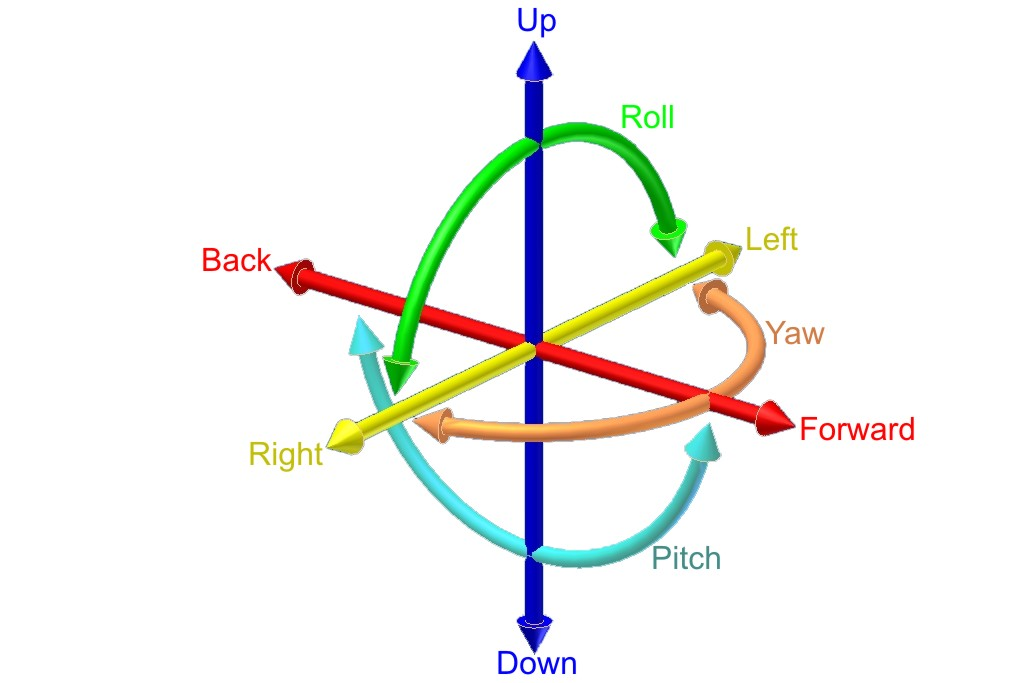
\includegraphics[width=0.3\textwidth]{imgs/ejesdrone.eps}
		\caption{Esta imagen muestra los movimientos que tiene un dron.}
	\label{fig:ejesdrone}
\end{figure}

\hspace{1 cm} Explicado esto, un desglose explicando cada una de las partes ser\'ia :

\hspace{1 cm}\textbf{Frame:} Tambi\'en conocido como marco, estructura o chasis. Es la estructura principal sobre la que se situan el resto de los elementos. Este variar\'a su forma dependiendo del dron, variando la longitud de las patas o el n\'umero de soportes para helices, por ejemplo. Esta puede estar hecha por diversos materiales, generalmente se trata de alg\'un tipo de plastico, ya que es un material que tiene poco coste y pesa poco. Un ejemplo es el polipropileno, que es ligero y con mucha resistencia, lo que permite colocar sobre el la bater\'ia. Otro material que suele utilizarse es la fibra de carbono, ya que se trata de un material que pesa poco y es muy resistente, aunque puede tener factores negativos como su conductividad. Por ultimo, tambi\'en nombrar la fibra de v\'idrio. Este material tambi\'en es muy utilizado por ser ligero, y tiene caracter\'isticas como que no es conductor de la electricidad. Es com\'un ver estucturas h\'ibridas entre distintos materiales, sobre todo juntando los dos tipos de fibra. 

\hspace{1 cm}\textbf{H\'elices:} Elemento formado por dos palas montadas de forma concentrica sobre un eje, que al girar crean un par de fuerzas, permitiendo as? el movimiento del dron.

\hspace{1 cm}\textbf{Motores:} Son los encargados de transformar la energ\'ia que llega en movimiento sobre el eje en el que se situan las h\'elices, para asi permitirles a estas hacer su trabajo. Este a su vez tiene distintos parametros que ser\'an principalmente los que permitan al drone llevar mayor velocidad. 

\hspace{1 cm} El numero de vueltas que d\'e por minuto, lo que dependera de los KiloVoltios. Este suele estar en torno a 800-900kV.

\hspace{1 cm} El tama?o que \'este tenga. Al mirar las especificaciones de un drone est\'a en un numero de 4 d\'igitos, en el que los dos primeros hacen referencia al tama?o del rotor y los otros dos al tama?o de la bobina. 

\hspace{1 cm} El empuje, valor que hacer referencia al peso que puede levantar el motor.

\hspace{1 cm} La corriente, que se trata de la energ\'ia (amperios) que se consume cuando el motor esta al m\'aximo.


\hspace{1 cm}\textbf{Bateria:} Encargada de proporcionar la energ\'ia suficiente para que el dron pueda realizar un vuelo, permitiendo trabajar a la placa controladora y motores. La caracter\'istica principal de las baterias son los miliamperios, ya que es la que permitir\'a una mayor capacidad y por lo tanto que el dron tenga un mayor tiempo de vuelo. Existen bater\'ias de muy diversos tama?os, desde los 350 mah en drones de jugete a, por ejemplo, los 4500mah que tiene la bater\'ia del dron 3DR solo. Tambi\'en es importante la tasa de descarga, que se trata de la m\'axima energ\'ia que puede entregar y el periodo de tiempo durante el que puede hacerlo. Normalmente los drones traen sitemas de alerta que avisan cuando a la bater\'ia le queda poca energ\'ia, o que cuando queda un valor menor a cierto porcentaje de carga no permite despegar el dron, evitando as\'i que se quede sin energ\'ia a mitad de un vuelo.

\hspace{1 cm}\textbf{Equipo de transmision:} Es el encargado de que se comunique el dron con una estaci\'on receptora. Este puede variar en funcion del aparato ya que se pueden usar diferentes tecnolog\'ias, pero principalmente se trata de radiofrecuencia o de Wifi. Existen casos, como el modelo 3DR que combina ambas tecnolog\'ias, utilizando la radiofrecuencia para la informaci\'on del movimiento, bater\'ia y posicionamiento, y el WiFi para la transmisi\'on de im\'agenes en directo. Podemos encontrar distintos equipos de sistemas de transmisi\'on, uno de los ultimos y mas destacables es \textbf{Hyperion}, que utiliza un sistema \'optico de comunicaciones capaz de transmitir hasta 1Gb por segundo, lo que permite la transmisi\'on de datos mediante la luz directa. La principal caracter\'istica de \'este es que no pierde informaci\'on cuando no hay contacto directo entre las dos estaciones. Pero v\'ia WiFi es algo muy utilizado en los ultimos momentos, pues permite controlar el dron desde una aplicaci\'on movil, por lo que conectando estos dos tendr\'iamos un mando que nos permite cambiar gran parte de la configuraci\'on del dron. Tambi\'en existen dispositivos que permiten el control mediante Bluetooth, pero este es menos com\'un ya que tiene mayor restricci\'on de velocidad de datos y distancia. 


\hspace{1 cm}\textbf{Placa controladora:} Es el procesador del dron, el que se encarga de recoger la informaci\'on del dron y cuando le llega una orden ver que informaci\'on tiene que mandar para que \'esta se ejecute de forma correcta, as\'i como en caso de haber un problema tratar de evitarlo. Este es basicamente el hardware que utiliza el dron, hay una gama muy amplia dentro de \'este,donde cabe destacar \textbf{Pixhawk},pero podemos encontrar varias con gran trascendencia: 
	\begin{itemize}
		\item Pixhawk: Este es el m\'as utilizado debido a que trabaja con 3DRobotics y Ardupilot. Este sirve para diversos dispositivos como son drones, helic\'opteros y barcos. Esta pensado para cualquier veh\'iculo que tenga movimiento.  Se trata de un proyecto hardware abierto, cuyo objetivo principal es proporcionar el hardware de autopiloto a comunidades acad\'emicas o gente que tiene esto como un hobby, teniendo as\'i un bajo costo y una alta disponibilidad. Se trata de un piloto autom\'atico en tiempo real y muy eficiente, proporcionando un entorno de estilo POSIX. Este es el autopiloto estandar de la industria, y por lo tanto, como veremos a continuaci\'on, a partir del cual se han desarrollado diversos autopilotos con distintas mejoras. 

		\item Pixhawk2: Es una versi\'on avanzada de la placa anterior. Este tiene mejoras como aislamiento de vibraciones, 3 IMUs para redundancia(3 acelerometros, 3 giroscopios, 3 magnetometros y 2 barometros) y sensor para controlar la temperatura. 

		\item PixRacer: \'Este se ha desarrollado para los drones de carreras, aunque tambi\'en se utiliza en minidrones. Suele tener una mayor memoria flash.

		\item Navio2: Piloto autom\'atico dise?ado de Raspberry Pi. Te permite convertir esta en un controlador de drone. 

		\item PXFmini: Se trata de otro piloto autom\'atico de Raspberry Pi. Este tiene la electr\'onica para la mayoria de los componentes que puede utilizar un dron. 

		\item FlytPOD: Este se trata de una placa Odroid XU4 SBC junto con una PixHawk. Puede volar diversos veh\'iculos aereos y su principal caracter\'istica es el WiFi que tiene integrado. Existe una placa FlytPOD pro que se trata de una versi\'on extendida de la anterior, teniendo todas sus caracter\'isticas, pero con mas sensores y mayor capacidad de almacenamiento. 

		\item U-Pilot: Este hardware se caracteriza por servir para diversos vehi\'iculos aereos, siendo programable para realizar todas las acciones de su camino de forma autom\'atica. Su radioenlace con frecuencia en torno a 900Mhz permite controlar el dispositivo a una distancia de 100km. 
	\end{itemize}

\hspace{1 cm} Hay que destacar un elemento impotante como es la \textbf{camara}, que aunque no todos los drones la llevan s\'i que es algo bastante com\'un. Algunos la llevan incorporada (incluso dos camaras, una que apunta hacia la parte de delante y otra que apunta la parte de abajo) y otras que traen soporte para poder incorporar ciertas camaras, normalmente consideradas camaras de acci\'on, para as\'i obtener una mejor calidad, e incluso incorporar adaptadores como puede ser una Gimbal para controlar la parte hacia la que queremos que apunte la camara en cada momento o utilizarlo como estabilizador, para evitar asi que afecten a la imagen diversos movimientos, generalmente bruscos, que pueda realizar el dron. Cabe destacar que en muchas ocasiones, utilizado normalmente para carreras de drones, la c\'amara sirve para integrar la tecnolog\'ia FPV (First Person View), que es junto a la c\'amara, el transmisor de v\'ideo y el receptor de v\'ideo, poder ver en tiempo real las imagenes sobre una pantalla LCD o utilizando unas gafas de realidad virtual. En este aspecto, en los ultimos a?os se ha visto por otro lado un gran avance de la realidad virtual, y es tambi\'ien hay una gran variedad en este mundo, pues existe una gama que va desde las \emph{cardnboard}, que permiten con un trozo de cart\'on y un par de lentes, poniendolos de cierta forma y con el uso de un smartphone, tener de forma sencilla unas gafas 3D, hasta gafas para la videoconsola que te permiten entrar en el videojuego, a?adiendo una gran calidad de imagen y con un sonido envolvente para entrar de lleno en el ambiente. Pero una de las cosas mas impactantes es el conjunto que se ha creado con el done \textbf{FLYBi}, estando \'este conectado a unas gafas de realidad virtual que tienen sensor de movimiento, lo que te permite sentir que eres t\'u el que vuelas y el que est\'as en el lugar del dron, y con cualquier movimiento que sientan las gafas la c\'amara del drone lo imitar\'a. En caso de que esto parezca incomodo el dron tiene un joystick con el que enviar\'a la informaci\'on de los elementos a realizar a la c\'amara. 
 

\begin{figure}[H]
 \centering
  \subfloat[Chasis]{
   \label{f:chasis}
    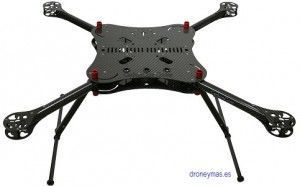
\includegraphics[width=0.2\textwidth]{imgs/chasis-drone.jpg}}
  \subfloat[Helices]{
   \label{f:helices}
    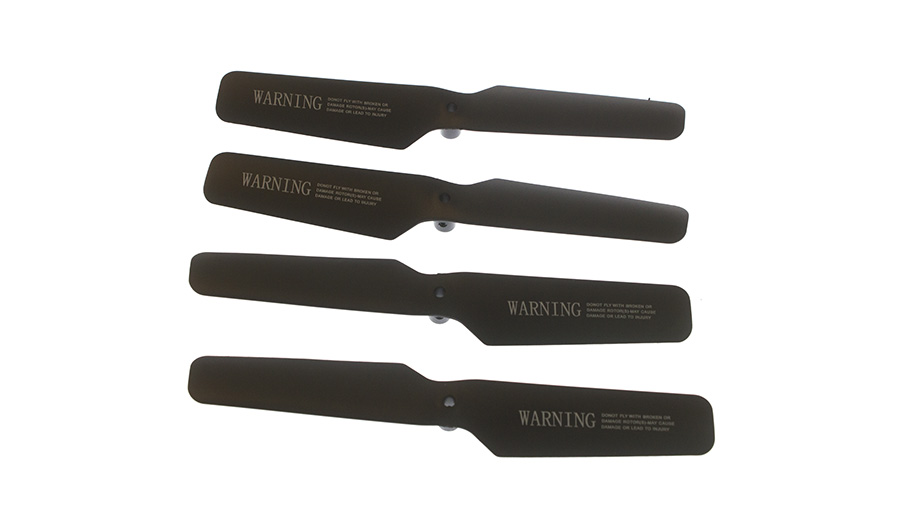
\includegraphics[width=0.2\textwidth]{imgs/helices-drone.jpg}}
  \subfloat[Motor]{
   \newline\label{f:motor}
    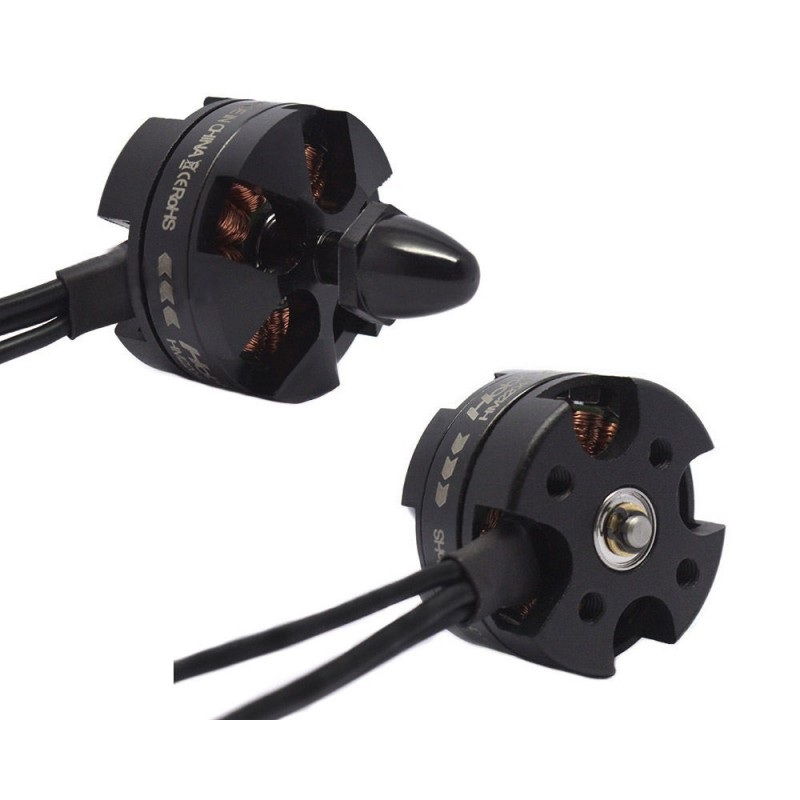
\includegraphics[width=0.2\textwidth]{imgs/motor-drone.jpg}}
	\subfloat[Placa-Madre]{
   \newline\label{f:placa-madre}
    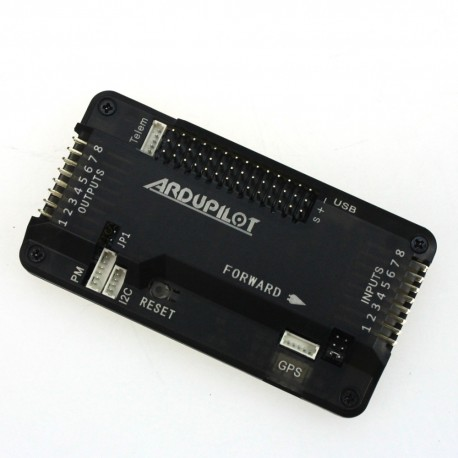
\includegraphics[width=0.2\textwidth]{imgs/placaControladora-drone.jpg}}
 \caption{Distintas partes del drone.}
 \label{f:Test 1}
\end{figure} 


\section{Software.}
\hspace{1 cm} Como sabemos, el software es el conjunto de programas que van a permitir realizar ciertas tareas, en este ser\'a lo que permita realizar al drone una navegaci\'on aut\'onoma. Dicho programa estar\'a instalado en la placa controladora, y por tanto sera el que ejecute para recoger la distinta informaci\'on de los sensores, procesar la informaci\'on y enviar las ordenes correctas a los distintos elementos de este. Como se ha comentado anteriormente, el desarrollo de software para este tipo de robots ha evolucionado mucho en los ultimos años debido al uso civil que se le comienzan a dar y no tanto al desarrollo militar. Es importante destacar el software de \textbf{ArduPilot}, ya que se trata del software auto-piloto mas avanzado, pero existen tambi\'en otros que nos permiten el manejo de estos robots:

	\begin{itemize}
		\item \textbf{Ardupilot:} Es un sistema OpenSource encargado de recibir la informaci\'on que se le da y de esta forma enviar las señales correspondientes a los actuadores. Se trata del software mas importante debido a lo completo que es y confiabilidad que proporciona,debido a la gran cantidad de gente que lo utiliza(pilotos de drones profesionales y aficionados) y por el equipo de ingenieros que lo ha desarrollado. Este software se caracteriza por la variedad de dispostivos que puede llegar a controlar, ya que trabaja con diversos dispositivos aereos(aviones, helicopteros, drones, etc) y con dispositivos marinos(como pueden ser los barcos y submarinos). Este ha tenido un gran desarollo debido a su principal caracter\'istica: Opensource. Hay mucha gente creando interfaces para este y dichos usuarios comparten sus avances con el resto. A partir de \'este han nacido controladores como Ardupilot Mega. El problema que tiene dicho software es que solo permite trabajar con plataformas de los mismos creadores, lo que lleva al siguiente software. Otra caracter\'istia es la facilidad con la que se le pueden añadir diferentes sensores, como pueden ser modulos GPS o camaras, algo que facilitar\'a la navegaci\'on aut\'onoma. 

	\item \textbf{Megapirate-NG:} Apareci\'o como desarrollo del anterior. La funcionalidad de uno y otro es practicamente la misma, con la diferencia de que \'este permite trabajar con Hardware de otros creadores. El problema es que siempre depende de Ardupilot, por lo tanto sus funcionalidades, aunque sean mas c\'omodas para trabajar, puede que esten atrasadas.

		\item \textbf{MultiWii:} \'Este se propuso como radiocontrol para drones. Es un sistema que fue creado por los desarrolladores y con los sensores (giroscopios y acelerometros) de la Nintendo Wii. Es una plataforma basada en arduino, con el factor en contra de tener una funcionalidad bastante limitada. 
	\end{itemize}


Estos primeros son los softwares principales que estar\'ian sobre el veh\'iculo, pero tambi\'en estan los programas que se ejecutar\'ian en otros dispositivos como el ordenador o el tel\'efono m\'ovil para ver la informaci\'on que este nos env\'ia. Normalmente el fabricante del drone tiene ya un programa que realiza esta funci\'on. 

\hspace{1 cm} En este punto es importante el protocolo de comunicaci\'on que habr\'a para comunicarse el veh\'iculo con la estaci\'on terrena. Aqu\'i hay un protocolo que destaca sobre los dem\'as, el \textbf{MAVLink} (Micro Air Vehicle Communication Protocol). \'Este protocolo tiene la informaci\'on contenida en ficheros .xml, lo que permite utilizarlo en diversos lenguajes de comunicaci\'on, lo que conlleva una mejora notable en su desarrollo. Al tener el fichero .xml los tipos de mensaje, permite con facilidad a?adir nuevos tipos para asignar una tarea nueva a cada uno. Otra ventaja de este es que hay muchos software de drones que lo soportan, como pueden ser Ardupilot, Autopilot, algunos derivados de estos y otros como Gentlenav o Flexipilot, y desde la estaci\'on tierra algunos como MAVProxy, Mission Planer o APM planner. 
Un problema en este protocolo es que los datos no estan encriptados en la comunicaci\'on, por lo que es mas facil un ataque y que se manipulen los datos, siendo detectable si se hace perder algun dato ya que se utiliza CRC (codigo de redundancia c\'iclica para detectar cambios en los datos, este se utiliza en protocolos como TCP).
MAVLink utiliza otro software llamado MAVProxy para poder acceder a los datos del veh\'iculo, como la velocidad y las im\'agenes, lo que nos permitir\'a tambi\'en saber que datos mandarle para que funcione de forma correcta. 

\hspace{1 cm} A parte de todos estos, existen tambi\'en otras infraestructuras software como puede ser \textbf{JdeRobot}. En s\'i JdeRobot se trata de un software de desarrollo para rob\'otica y aplicaciones de visi\'on por computador. \'Este puede trabajar con distintos sensores que le proporcionan informaci\'on, en caso del drone con la informaci\'on que le permite Ardrone Server, y gracias a esto puede controlar el dispositivo y ver los distintos datos de este. Con JdeRobot es muy sencillo tomar el control del hardware gracias a su programa de control. Tiene una gran API que permite realizar diversas tareas como trabajar con aparatos reales o simulados, y conectarse a ellos de forma local o a trav\'es de la red. Decir que para el trabajo realizado, esta plataforma ha sido muy importante, pues su componente para la c\'amara, su aplicaci\'on para filtros de color y la posibilidad de realizar diagramas de estado permite tener en todo momento datos importantes del dron y poder mantenerlo bajo control sin ningun problema. Destacar que se trata de un sistema OpenSource que permite trabajar con simuladores como Gazebo y con ayuda de librerias como OpenCV. 
 

\hspace{1 cm} A parte de todos estos, existen tambi\'en otras infraestructuras software como puede ser \textbf{JdeRobot}. En s\'i JdeRobot se trata de un software de desarrollo para rob\'otica y aplicaciones de visi\'on por computador. \'Este puede trabajar con distintos sensores que le proporcionan informaci\'on, en caso del drone con la informaci\'on que le permite Ardrone Server, y gracias a esto puede controlar el dispositivo y ver los distintos datos de este. Con JdeRobot es muy sencillo tomar el control del hardware gracias a su programa de control. Tiene una gran API que permite realizar diversas tareas como trabajar con aparatos reales o simulados, y conectarse a ellos de forma local o a trav\'es de la red. Decir que para el trabajo realizado, esta plataforma ha sido muy importante, pues su componente para la c\'amara, su aplicaci\'on para filtros de color y la posibilidad de realizar diagramas de estado permite tener en todo momento datos importantes del dron y poder mantenerlo bajo control sin ningun problema. Destacar que se trata de un sistema OpenSource que permite trabajar con simuladores como Gazebo y con ayuda de librerias como OpenCV. 
 
\hspace{1 cm} Ya que este proyecto se ha desarrollado en python, hay que destacar algunas librerias y herramientas muy importantes para la creaci\'on de un buen software, lo que permitir\'a una mejor y m\'as r\'apida ejecuci\'on. 
	\begin{itemize}
	\item OpenCV: Se trata de una biblioteca de visi\'on artificial. Esta biblioteca est\'a implementada en C++, pero se puede utilizar en los distintos lenguajes como C++,C, python y Java. Es una biblioteca utilizada por miles de usuarios y tiene funciones que te permiten detectar movimiento, reconocer objetos, reconocimiento facial y trabajar sobre im\'agenes (modificando datos de \'estas), mostrando, guardando y creando nuevas im\'agenes, cambios de valor sobre pixeles concretos para que sea mas sencillo ver el proceso que se esta realizando. Est\'a disponible para los diversos sistemas operativos y se utiliza mucho para software de visi\'on. Se trata de una librer\'ia opensource y por lo tanto su desarrollo puede avanzar a gran velocidad ya que todo el mundo puede contribuir y compartir este.
	
	\item PIL: Esta librer\'ia permite la edici\'on de im\'agenes desde python. Tiene una gran variedad de operaciones que permite el realizar diversos cambios como puede ser rotaci\'on, escalado o manipulaci\'on de p\'ixeles en imagenes, adem\'as de cargar y guardar estas para trabajar con ellas o una vez est\'en modificadas. 
	
	\item NumPy: Se trata de un paquete en python que permite la computaci\'on cient\'ifica. La principal caracter\'istica son las matrices multidimensionales que permite hacer y el conjunto de funciones matem\'aticas que tiene para poder operar. NumPy permite ejecutar a gran velocidad las operaciones deseadas. En ocasiones los datos obtenidos en operaciones con la biblioteca OpenCV son almacenados en matrices NumPy, pues en realidad estas im\'agenes son matrices de datos a las que se le dan ciertos valores para luego poder representarlas, y acceder a estas estructuras se puede hacer de forma mas sencilla con un bajo coste computacional, adem\'as de permitirte interoperabilidad con otros paquetes como scipy o matplotlib. 

	\item Scipy: Esta librer\'ia Opensource permite trabajar con diversos algoritmos matem\'aticos de gran capacidad ya que tiene modulos para la optimizaci\'on de funciones. 
	\end{itemize}
	
	Cabe destacar las diferencias que tiene este lenguaje de programaci\'on respecto a otros. La principal diferencia es que se trata de un lenguaje interpretado, por lo que podriamos decir que sus programas hacen una compilaci\'on en directo, es decir que mientras compilan ejecutan, lo conlleva que no haya errores de compilaci\'on sino que sean errores en ejecuci\'on. Este tiene ventajas como la simplicidad para escribir el codigo, ya que te permite hacerlo de forma mucho mas limpia y abreviada que en otros lenguajes. No te obliga a declarar el tipo del que es una variable, simplemente con asignarle un valor ya te deja trabajar con el, a diferencia de otros como C o Java que si hay que declararlo. Todo esto conlleva que el tiempo de desarrollo en un programa se reduce de forma notable, permite que sea mejor y mas fluido el trabajo en equipo ya que si se crea un codigo legible es mas facil de entender y te permite no estar preocupado por la reserva y liberaci\'on de memoria. Tiene tambi\'en factores en contra como pueden ser el rendimiento, pues para hacer la misma operaci\'on necesita mas tiempo que otros lenguajes, y emplea mas memoria. Destacar que se esta trabajando en esto ya que se considera una desventaja importante, y se han creado herramientas como \textbf{Numba}, que con pocas lineas permite que este acelere su ejecuci\'on, hasta veinte veces su velocidad. 
	
	
\section{Uso actual de los drones}
\hspace{1 cm} Teniendo ya el contexto de las distintas caracter\'isticas que tiene un drone, se va a proceder a describir los distintos usos que se le pueden dar a estos. Cabe destacar que esto compende distintos campos y todos muy diversos, por lo que al principio se van a comentar los usos que mas se ven en la sociedad en general para terminar viendo usos mas especificos de la rob\'otica aerea, concretamente los que llevan a que este pueda trabajar de manera aut\'onoma. 

\subsection{Medios Audiovisuales.}
\hspace{1 cm} El drone es un elemento que se ha incorporado ultimamente en este sector debido a la camara que pueden tener. Gracias a esto permite tomar planos de ciertas zonas o fotografias que ser\'ian muy dificil de obtener en condiciones normales. Tambi\'en se debe a que el precio de estos es asequible, por lo que se puede acceder a ellos con facilidad,y en un sector tan amplio y vistoso como es este, lleva a un uso cada vez mas com\'un.

\subsection{Control de distintas zonas.}
\hspace{1 cm} En este area podemos destacar varios usos distintos, pero su expansi\'on en esto se debe a que con un drone podemos controlar una zona para la que anteriormente necesitabamos varias camaras, y aun asi podian quedar zonas sin vigilar. Esta tecnolog\'ia nos lleva a poder mover una camara por un lugar amplio sin necesidad de estar alli ni de tener un gran despliegue de elementos, asi como evitar que queden puntos muertos. Algunos ejemplos de esto son los siguientes: 


\begin{itemize}
	\item\textbf{Seguridad:} Teniendo un drone en un lugar como pueda ser una nave industrial, podemos hacer que este se desplace grabando en todo momento lo que ve, y si se detecta algo sospechoso en alg\'un lugar el drone se diriga all\'i en el momento para obtener im\'agenes de lo que esta pasando. 
	
	\item \textbf{Sector agr\'icola:} Se debe a la facilidad con la que un drone puede sobrevolar una zona y ofrecer imagenes de alta calidad de esta, obteniendo un buen control de los cultivos en menos tiempo, con menos gasto y al tratarse de un vehiculo electrico al evitar desplazamientos de otros automoviles conlleva un menor impacto ambiental. Adem\'as, este permite ver con facilidad el estado de la cosecha, detectar enfermedades o plagas, permiten fumigar desde el aire con mayor precisi\'on, ya que les puedes programar una ruta y que sigan esta. Tambi\'en podrian obtener otros datos como las zonas con mas y menos agua, y obtener las condiciones del terreno y ver si son optimas para esperar cierto resultado.
	
	\item \textbf{Mantenimiento:} En este apartado podemos englobar diversas actividades, como puede ser mantenimiento de edificios y construcciones, redes electricas o diversas instalaciones industriales como aerogeneradores e\'olicos y estados de paneles solares. Al igual que en el apartado anterior, aqui podemos recorrer grandes distancias, por ejemplo para comprobar las redes electricas, sin la necesidad de que un operario pierda mucho tiempo recorriendo dicha l\'inea. Con las instalaciones solares por ejemplo, desde un plano superior podriamos observar si todas las placas estan en las condiciones optimas y en caso de existir algun fallo poder identificarlo con facilidad. Para edificios y aerogeneradores lo que hay que tener en cuenta es la altura que estos pueden tener, y a la cual con un dron llegar\'iamos con facilidad y observar\'iamos si hay algun problema. En estos casos lo que evitamos, como anteriormente he comentado, es que alguien tenga que ir sitio a sitio perdiendo mucho tiempo. Destacando tambi\'en que este tipo de actividades se pueden implementar programas que directamente detecten las anomalias, sin necesidad de que haya una persona revisando en todo momento las im\'agenes, donde tambi\'en con una inversion inicial, al final ahorrariamos mucho tiempo y dinero. 
\end{itemize}

\hspace{1 cm} Por otro lado, pueden aportar gran ayuda en situaciones que no se dan de forma peri\'odica, sino que ocurren de forma espor\'adica y en lugares muy distintos. Gracias a los drones podemos tener una camara que nos muestre una imagen de esta zona o que nos permita ayudar all\'i, y en otro momento llevarlo a otro lado, lo que lleva a no tener un gran despliegue de medios en un lugar que apenas va a ser necesario. Los ejemplos podrian ser los siguentes:

\begin{itemize}
	\item \textbf{Emergencias:} Cuando ocurren ciertas catastrofes naturales por ejemplo, son de gran ayuda debido a la velocidad con la que pueden llevar materiales (medicos o de otro tipo) a la zona afectada.

	\item \textbf{Busqueda de personas:} Al tratarse de medios que pueden sobrevolar zonas obteniendo grandes im\'agenes, pueden ser de ayuda cuando monta?eros o caminantes tienen accidentes en bosques o monta?as, quedan incomunicados y se comienza una b\'usqueda.

	\item \textbf{Incendios forestales:} Los drones pueden estar sobrevolando zonas y obteniendo informaci\'on de esta, para as\'i poder prevenr posibles incendios o alertar lo antes posible en cuanto uno ocurra. 

\item \textbf{Investigaciones:} Para este apartado pueden ser de distinto tipo, ya que puede recorrer zonas largas de restos arqueologicos y tomar datos de estos, entrar en zonas peligrosas como ciertas cuevas o volcanes y obtener datos para su posterior estudio, e incluso investigaciones biologicas, recreando en un dron la actividad de un ave para as\'i estudiar su comportamiento.
\end{itemize}

\subsection{Desarrollo aut\'onomo.}
\hspace{1 cm} Es muy importante este ambito, pues determinados grupos y grandes empresas estan trabajando en su desarrollo debido al futuro que se viene por delante. Esto se debe a la facilidad que puede llevar esto para realizar grandes tareas, como el control de material en almacenes o transporte de material de un lugar a otro. Una c\'aracteristica importante es la rapidez con la que pueden llegar los drones de un lugar a otro, y acceder a lugares que es dificil por otros vehiculos. A continuaci\'on se muestran distintos usos que estan aplicando sobre estos grandes empresas. 


\hspace{1 cm} Por un lado, como pionero en este area se encuentra \textbf{Amazon}, el cual lleva desarrollando desde 2013 una tecnolog\'ia que permita el reparto de paquetes mediante drones. Esta tecnolog\'ia lleva consigo los llamados almacenes aereos, es decir, un almacen que se mantendria en el aire gracias a dirigibles, el cual tiene paquetes a entregar y drones. El drone obtendria el paquete que se debe entregar y lo llevar\'ia al lugar adecuado. Tras esto volver\'ia a un almacen hasta que se le mande de nuevo al almacen aereo para el siguiente reparto. Estos drones sabr\'ian en todo momento en el estado y en el punto en el que se encuentran, es decir, que saben a que lugar deben ir dependiendo de la tarea a realizar. 

\begin{figure}[ht]
	\centering
		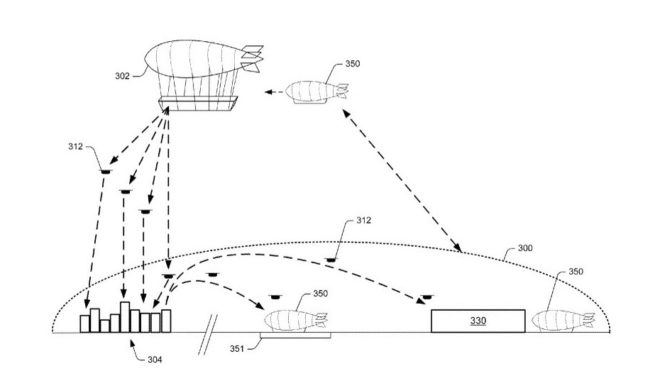
\includegraphics[width=0.55\textwidth]{imgs/amazon.jpg}
	\label{fig:Esquema de reparto con drones}
\end{figure}

\hspace{1 cm} Por otro lado, tambi\'en para el reparto de mercancias se encuentra \textbf{Google}, este empez\'o sus pruebas en 2014 y tuvo un programa piloto en Australia, pero no consiguio llevarlo a Estados Unidos. Aun as\'i, consiguio hacer pruebas en una universidad de reparto de comida, un reto que supuso principalmente que la comida llegara rapido a su destino y en buenas condiciones.Adem\'as tambi\'en sirvi\'o para ajustar los sistemas autom\'aticos de vuelo y entrega de la mercancia. 

\hspace{1 cm} A raiz de estos servicios de entregas, se ha producido otro desarrollo importante, como puede ser el de tener controlados los paquetes dentro de un almacen. Un pionero de esto ha sido un grupo en el \textbf{MIT}, desarrollando un sistema que permite a los drones moverse por los almacenes escaneando los codigos de cada paquete, enviando esta informaci\'on a un servidor y que este pueda tener controlados los paquetes que hay y donde estan situados. 

\hspace{1 cm} Para el traslado de mercancias en interiores tambi\'en se ha puesto en marcha la cadena de supermercados estadounidense Walmart, cuyo objetivo es transportar productos de un lugar a otro previamente establecidos. La idea de este proyecto se debe a los grandes almacenes que tienen estos supermercados, y que cuando un cliente no encuentra el producto deseado, avisa a un empleado y este tiene que ir al almacen a buscarlo, perdiendo mucho tiempo entre la distancia recorrida y la busqueda del producto. Lo que conseguirian con esto, es que en caso de que los empleados esten ocupados, un cliente no tenga que estar a la espera, sino que con un dispositivo podamos pedir el producto y un drone se encargar\'a de ir a por el y traerlo al punto donde nos encontremos. Destacar que se incorporaran en las tiendas controladores aereos para que los vehiculos sigan una trayectoria segura.  

